\documentclass[spanish,12pt,a4paper,titlepage]{report}
\usepackage[utf8]{inputenc}
\usepackage{graphicx}
\usepackage{subfig}
\usepackage{float}
\usepackage{wrapfig}
\usepackage{multirow}
\usepackage{caption}
\usepackage[spanish]{babel}
\usepackage[dvips]{hyperref}
\usepackage{amssymb}
\usepackage{listings}
\usepackage{epsfig}
\usepackage{amsmath}
\usepackage{array}
\usepackage[table]{xcolor}
\usepackage{multirow}
\usepackage[Sonny]{fncychap}
%\usepackage[Lenny]{fncychap}
%\usepackage[Glenn]{fncychap}
%\usepackage[Conny]{fncychap}
%\usepackage[Rejne]{fncychap}
%\usepackage[Bjarne]{fncychap}
%\usepackage[Bjornstrup]{fncychap}

%\usepackage{subfiles}
%\usepackage{framed}

\usepackage{color}
\newcommand{\highlight}[1]{\colorbox{yellow}{#1}}    %\highlight{this is some highlighted text}
\newcommand{\highlightdos}[1]{\colorbox{green}{#1}}    %\highlight{this is some highlighted text}

\setlength{\topmargin}{-1.5cm}
\setlength{\textheight}{25cm}
\setlength{\oddsidemargin}{0.3cm} 
\setlength{\textwidth}{15cm}
\setlength{\columnsep}{0cm}


\begin{document}

\chapter{Arranque Quad}

Como hablamos ayer, sniffié todo el arranque desde un poquito antes de prender el botón hasta un poco después que los motores empezaron a funcionar. Sniffié en tandas de 3 segundos sobreponiendo la última parte de uno con la primera del siguiente, como quedamos.\\
Fueron en total 5 sniffeadas.\\
Van todas las palabras que reconoció el sniffer en el orden adecuado:

\section*{Parte 1}

En esta parte las líneas permanecen todo el tiempo en Vcc, como se muestra en la figura \ref{fig:chrono}.

\begin{figure}[h!]
	\centering
	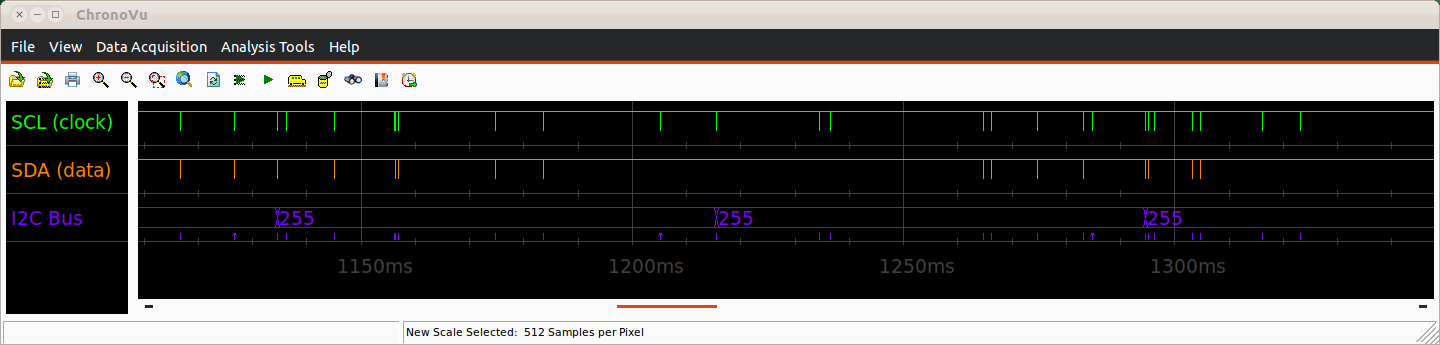
\includegraphics[width=0.99\textwidth]{./Pics/chrono.png}
	\caption{Sniffer}
	\label{fig:chrono}
\end{figure}

En esa imagen se puede ver también que tanto la línea de Clock como la de Datos bajan a 0 en algunos instantes. Este fenómeno parece ser esporádico y aleatorio. Supongo que se debe a errores de sniffeado...\\
El tema es que hacen que el sniffer se piense que se está enviando un 255. Lo que pasa es que interpreta esos cambios en las líneas como una secuencia de inicio y luego interpreta que se están mandado ``1s'' lógicos, formando el 255.\\
Yo creo que se deben interpretar los 255s como inactividad en el bus (quedan las líneas altas).\\
Acá van todas las palabras detectadas:

\begin{verbatim}
255   255   255   255   255   255   255   255   255   255   255   255
\end{verbatim}
\begin{verbatim}
255   255   255   255   255   255     0
\end{verbatim}

\section*{Parte 2}

\begin{verbatim}
255   255   255   255   255   255   255   255   255   255   255   255
\end{verbatim}
\begin{verbatim}
255     0
\end{verbatim}


\section*{Parte 3}

\begin{verbatim}
255   255   255   255   255   255   255   255   255   255   255   255
\end{verbatim}
\begin{verbatim}
255   255   255   255   255   255   255   255   255   255   255   255
\end{verbatim}
\begin{verbatim}
255   255   255   255   255   255     0
\end{verbatim}


\section*{Parte 4}

En la parte 4 termina de prender el quad. En el momento que hace el último pitido se ve en el sniffer un patrón como el que sigue:

\begin{verbatim}
||D2|A2|00||D4|A2|00||D6|A2|00||D0|A2|00||
\end{verbatim}

La representación gráfica es esta:

\begin{figure}[h!]
  \centering
  \subfloat[Potencia]{\label{fig:4P} 
  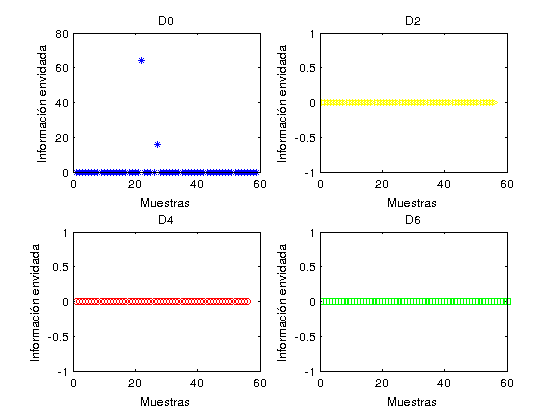
\includegraphics[width=0.55\textwidth]{./Pics/4P.png}}
  \subfloat[Registro]{\label{fig:4R} 
  		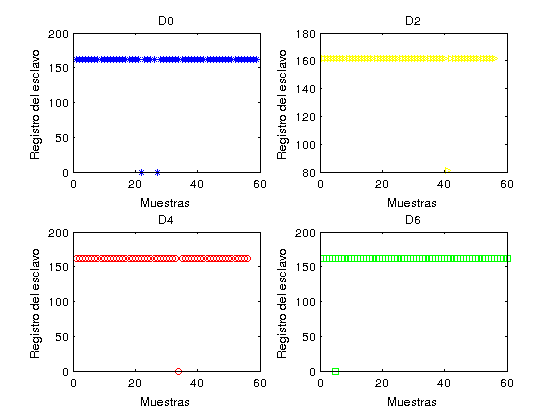
\includegraphics[width=0.55\textwidth]{./Pics/4R.png}}
  \caption{Parte 4}
  \label{fig:parte4}
\end{figure}


En la figura de la izquierda están las potencias enviadas a cada motor y en la de la derecha el valor del registro interno de cada esclavo.\\

Como el log es muy largo, lo pongo en un archivo aparte, que lo podés abrir haciendo clic \href{parte4.txt}{aca}. Si no anda el link, el archivo se llama parte4.txt y va adjunto.

\section*{Parte 5}

En esta parte termina de prender el quad y enseguida muevo la palanca del control, generando un escalón en los datos como se puede ver en la figura siguiente.\\

Cuando termina de prender empieza a tirar 0s. Muevo la palanca y aparecen las líneas inactivas por medio segundo aprox y luego empieza a tirar la potencia indicada por el control.\\

El log es más largo esta vez, y está \href{parte5.txt}{aca}. También lo podés abrir normal, también va adjunto.

\begin{figure} [h!]
  \centering
  \subfloat[Potencia]{\label{fig:5P} 
  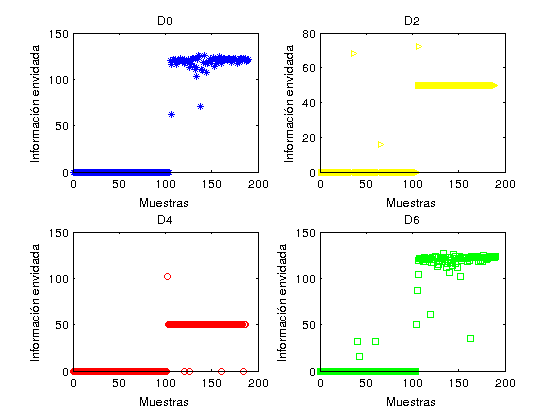
\includegraphics[width=0.52\textwidth]{./Pics/5P.png}}
  \subfloat[Registro]{\label{fig:5R} 
  		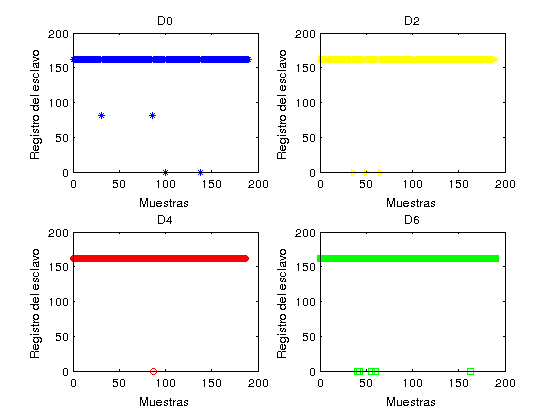
\includegraphics[width=0.52\textwidth]{./Pics/5R.png}}
  \caption{Parte 5}
  \label{fig:parte5}
\end{figure}

Más abajo están todas las imágenes más grandes

\newpage
\section{Imágenes grandes}
Van las imágenes más grandes para verlas mejor (por las dudas)

\begin{figure}[h!]
	\centering
	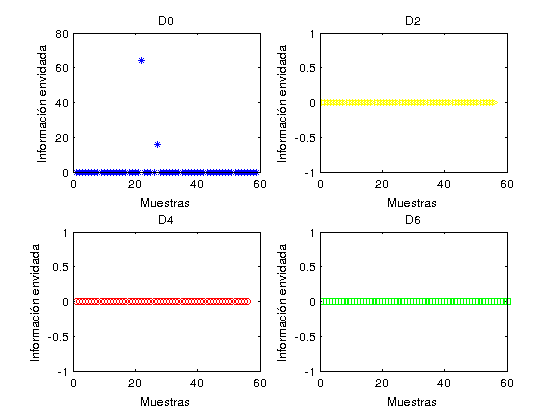
\includegraphics[width=0.9\textwidth]{./Pics/4P}
	\caption{Parte 4 - Potencia}
	\label{fig:}
\end{figure}

\begin{figure}[h!]
	\centering
	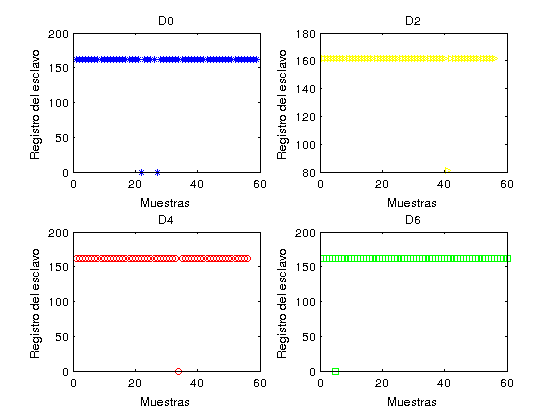
\includegraphics[width=0.9\textwidth]{./Pics/4R}
	\caption{Parte 4 - Registro}
	\label{fig:}
\end{figure}

\begin{figure}[h!]
	\centering
	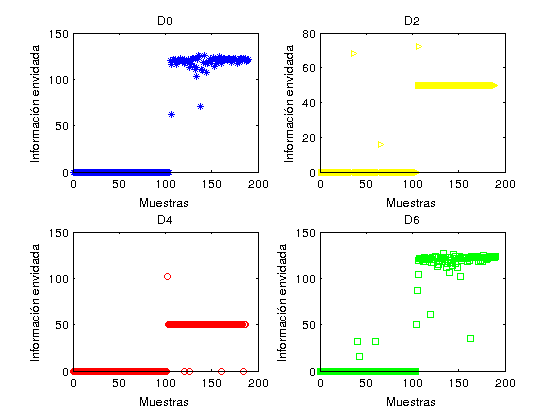
\includegraphics[width=0.9\textwidth]{./Pics/5P}
	\caption{Parte 5 - Potencia}
	\label{fig:}
\end{figure}

\begin{figure}[h!]
	\centering
	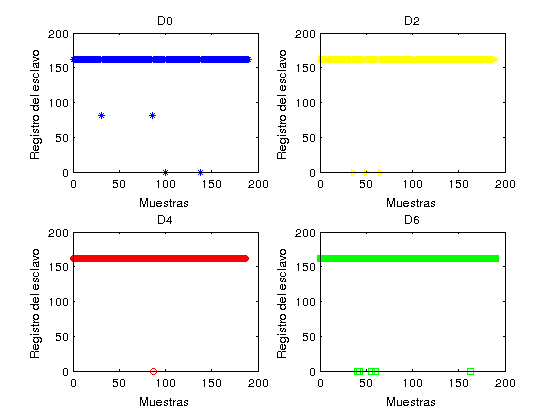
\includegraphics[width=0.9\textwidth]{./Pics/5R}
	\caption{Parte 5 - Registro}
	\label{fig:}
\end{figure}



\end{document}

